\documentclass{article}
%DIF LATEXDIFF DIFFERENCE FILE
%DIF DEL ../research-project-old/main.tex   Sun Jun 22 03:36:55 2025
%DIF ADD main.tex                           Sun Jun 22 05:05:36 2025
\pdfpagewidth=8.5in
\pdfpageheight=11in
\usepackage{ijcai20}

% Use the PostScript Times font!
\usepackage[nocompress]{cite}
\usepackage{times}
\renewcommand*\ttdefault{txtt}
\usepackage{soul}
\usepackage{url}
\usepackage[hidelinks]{hyperref}
\usepackage[utf8]{inputenc}
\usepackage[small]{caption}
\usepackage{graphicx}
\usepackage{amsmath}
\usepackage{booktabs}
\urlstyle{same}
\pagestyle{plain}
\setcounter{secnumdepth}{3}
%DIF PREAMBLE EXTENSION ADDED BY LATEXDIFF
%DIF UNDERLINE PREAMBLE %DIF PREAMBLE
\RequirePackage[normalem]{ulem} %DIF PREAMBLE
\RequirePackage{color}\definecolor{RED}{rgb}{1,0,0}\definecolor{BLUE}{rgb}{0,0,1} %DIF PREAMBLE
\providecommand{\DIFaddtex}[1]{{\protect\color{blue}\uwave{#1}}} %DIF PREAMBLE
\providecommand{\DIFdeltex}[1]{{\protect\color{red}\sout{#1}}}                      %DIF PREAMBLE
%DIF SAFE PREAMBLE %DIF PREAMBLE
\providecommand{\DIFaddbegin}{} %DIF PREAMBLE
\providecommand{\DIFaddend}{} %DIF PREAMBLE
\providecommand{\DIFdelbegin}{} %DIF PREAMBLE
\providecommand{\DIFdelend}{} %DIF PREAMBLE
\providecommand{\DIFmodbegin}{} %DIF PREAMBLE
\providecommand{\DIFmodend}{} %DIF PREAMBLE
%DIF FLOATSAFE PREAMBLE %DIF PREAMBLE
\providecommand{\DIFaddFL}[1]{\DIFadd{#1}} %DIF PREAMBLE
\providecommand{\DIFdelFL}[1]{\DIFdel{#1}} %DIF PREAMBLE
\providecommand{\DIFaddbeginFL}{} %DIF PREAMBLE
\providecommand{\DIFaddendFL}{} %DIF PREAMBLE
\providecommand{\DIFdelbeginFL}{} %DIF PREAMBLE
\providecommand{\DIFdelendFL}{} %DIF PREAMBLE
%DIF HYPERREF PREAMBLE %DIF PREAMBLE
\providecommand{\DIFadd}[1]{\texorpdfstring{\DIFaddtex{#1}}{#1}} %DIF PREAMBLE
\providecommand{\DIFdel}[1]{\texorpdfstring{\DIFdeltex{#1}}{}} %DIF PREAMBLE
\newcommand{\DIFscaledelfig}{0.5}
%DIF HIGHLIGHTGRAPHICS PREAMBLE %DIF PREAMBLE
\RequirePackage{settobox} %DIF PREAMBLE
\RequirePackage{letltxmacro} %DIF PREAMBLE
\newsavebox{\DIFdelgraphicsbox} %DIF PREAMBLE
\newlength{\DIFdelgraphicswidth} %DIF PREAMBLE
\newlength{\DIFdelgraphicsheight} %DIF PREAMBLE
% store original definition of \includegraphics %DIF PREAMBLE
\LetLtxMacro{\DIFOincludegraphics}{\includegraphics} %DIF PREAMBLE
\newcommand{\DIFaddincludegraphics}[2][]{{\color{blue}\fbox{\DIFOincludegraphics[#1]{#2}}}} %DIF PREAMBLE
\newcommand{\DIFdelincludegraphics}[2][]{% %DIF PREAMBLE
\sbox{\DIFdelgraphicsbox}{\DIFOincludegraphics[#1]{#2}}% %DIF PREAMBLE
\settoboxwidth{\DIFdelgraphicswidth}{\DIFdelgraphicsbox} %DIF PREAMBLE
\settoboxtotalheight{\DIFdelgraphicsheight}{\DIFdelgraphicsbox} %DIF PREAMBLE
\scalebox{\DIFscaledelfig}{% %DIF PREAMBLE
\parbox[b]{\DIFdelgraphicswidth}{\usebox{\DIFdelgraphicsbox}\\[-\baselineskip] \rule{\DIFdelgraphicswidth}{0em}}\llap{\resizebox{\DIFdelgraphicswidth}{\DIFdelgraphicsheight}{% %DIF PREAMBLE
\setlength{\unitlength}{\DIFdelgraphicswidth}% %DIF PREAMBLE
\begin{picture}(1,1)% %DIF PREAMBLE
\thicklines\linethickness{2pt} %DIF PREAMBLE
{\color[rgb]{1,0,0}\put(0,0){\framebox(1,1){}}}% %DIF PREAMBLE
{\color[rgb]{1,0,0}\put(0,0){\line( 1,1){1}}}% %DIF PREAMBLE
{\color[rgb]{1,0,0}\put(0,1){\line(1,-1){1}}}% %DIF PREAMBLE
\end{picture}% %DIF PREAMBLE
}\hspace*{3pt}}} %DIF PREAMBLE
} %DIF PREAMBLE
\LetLtxMacro{\DIFOaddbegin}{\DIFaddbegin} %DIF PREAMBLE
\LetLtxMacro{\DIFOaddend}{\DIFaddend} %DIF PREAMBLE
\LetLtxMacro{\DIFOdelbegin}{\DIFdelbegin} %DIF PREAMBLE
\LetLtxMacro{\DIFOdelend}{\DIFdelend} %DIF PREAMBLE
\DeclareRobustCommand{\DIFaddbegin}{\DIFOaddbegin \let\includegraphics\DIFaddincludegraphics} %DIF PREAMBLE
\DeclareRobustCommand{\DIFaddend}{\DIFOaddend \let\includegraphics\DIFOincludegraphics} %DIF PREAMBLE
\DeclareRobustCommand{\DIFdelbegin}{\DIFOdelbegin \let\includegraphics\DIFdelincludegraphics} %DIF PREAMBLE
\DeclareRobustCommand{\DIFdelend}{\DIFOaddend \let\includegraphics\DIFOincludegraphics} %DIF PREAMBLE
\LetLtxMacro{\DIFOaddbeginFL}{\DIFaddbeginFL} %DIF PREAMBLE
\LetLtxMacro{\DIFOaddendFL}{\DIFaddendFL} %DIF PREAMBLE
\LetLtxMacro{\DIFOdelbeginFL}{\DIFdelbeginFL} %DIF PREAMBLE
\LetLtxMacro{\DIFOdelendFL}{\DIFdelendFL} %DIF PREAMBLE
\DeclareRobustCommand{\DIFaddbeginFL}{\DIFOaddbeginFL \let\includegraphics\DIFaddincludegraphics} %DIF PREAMBLE
\DeclareRobustCommand{\DIFaddendFL}{\DIFOaddendFL \let\includegraphics\DIFOincludegraphics} %DIF PREAMBLE
\DeclareRobustCommand{\DIFdelbeginFL}{\DIFOdelbeginFL \let\includegraphics\DIFdelincludegraphics} %DIF PREAMBLE
\DeclareRobustCommand{\DIFdelendFL}{\DIFOaddendFL \let\includegraphics\DIFOincludegraphics} %DIF PREAMBLE
%DIF COLORLISTINGS PREAMBLE %DIF PREAMBLE
\RequirePackage{listings} %DIF PREAMBLE
\RequirePackage{color} %DIF PREAMBLE
\lstdefinelanguage{DIFcode}{ %DIF PREAMBLE
%DIF DIFCODE_UNDERLINE %DIF PREAMBLE
  moredelim=[il][\color{red}\sout]{\%DIF\ <\ }, %DIF PREAMBLE
  moredelim=[il][\color{blue}\uwave]{\%DIF\ >\ } %DIF PREAMBLE
} %DIF PREAMBLE
\lstdefinestyle{DIFverbatimstyle}{ %DIF PREAMBLE
	language=DIFcode, %DIF PREAMBLE
	basicstyle=\ttfamily, %DIF PREAMBLE
	columns=fullflexible, %DIF PREAMBLE
	keepspaces=true %DIF PREAMBLE
} %DIF PREAMBLE
\lstnewenvironment{DIFverbatim}{\lstset{style=DIFverbatimstyle}}{} %DIF PREAMBLE
\lstnewenvironment{DIFverbatim*}{\lstset{style=DIFverbatimstyle,showspaces=true}}{} %DIF PREAMBLE
%DIF END PREAMBLE EXTENSION ADDED BY LATEXDIFF

\begin{document}

\title{
    
\includegraphics[width=8cm, keepaspectratio]{tudelftlogo.png}\\
    \vspace*{2cm}
    \textbf{
         Benchmarking Geo-distributed Databases \\
         \large Evaluating Performance using the Product-Parts-Supplier Workload
    }\\
    \vspace*{1cm}
}

\author{
    \textbf{Eduard-Alex Mihai$^1$}\\
    \hfill \break
    \textbf{Supervisors: Asterios Katsifodimos$^1$, Oto Mráz$^1$}\\
    \break
%    \affiliations
    {\large 
        \hfill \break
        $^1$EEMCS, Delft University of Technology, The Netherlands
    }\\
}

\date{}

\maketitle
\thispagestyle{empty}

\let\clearpagebackup\clearpage
\renewcommand{\clearpage}{ }

\onecolumn

\vspace*{1.5cm}
\begin{center}
    A Thesis Submitted to EEMCS Faculty Delft University of Technology,\\
    In Partial Fulfilment of the Requirements\\
    For the Bachelor of Computer Science and Engineering\\
    \today
\end{center}

\vspace*{2cm}

\noindent
{\small
Name of the student: Eduard-Alex Mihai \\
Final project course: CSE3000 Research Project\\
Thesis committee: Asterios Katsifodimos, Oto Mráz, Koen Langendoen\\
}
\vfill

\begin{center}
    An electronic version of this thesis is available at http://repository.tudelft.nl/.
\end{center}

\twocolumn
\let\clearpage\clearpagebackup  
\clearpage
\setcounter{page}{1}


\begin{abstract}
\label{sec: abstract}
Existing evaluations of geo-distributed databases still rely almost exclusively on standard limited workloads such as TPC-C and YCSB+T, which reveal little information about the true cost of wide-area coordination. In this paper, we present a configurable benchmarking framework built around the Product-Parts-Supplier (PPS) workload, and use it to evaluate four representative systems that support geo-distributed transactions: Calvin, SLOG, Detock, and Janus. The experiments run across six realistic and insightful scenarios that vary the transactional load, contention, client count, regional bias, network latency, and packet loss.

The results uncover clear design trade-offs between the systems and demonstrate that our new framework is capable of filling several evaluation holes left by the standard workloads. Our framework introduces important features such as dependent transactions that may abort and retry, longer and tunable read/write sets, and fine-grained control over which regions will participate in the commit. However, the PPS workload comes with some limitations, and thus, the framework does not cover every case. As a consequence, for now, it should complement TPC-C and YCSB+T, not replace them.
\end{abstract}

\section{Introduction}
\label{sec: introduction}

In the modern era of cloud computing and real-time global services, geo-distributed databases have become essential to many critical large-scale applications \cite{corbett2013spanner, bronson2013tao}. These systems replicate and partition data across multiple geographical regions to provide high durability and significantly improve the latency by storing the data closer to the users. However, this distributed infrastructure comes with several tradeoffs. Given the high communication delays between different servers, it becomes increasingly challenging to synchronize transactions that access data scattered across multiple regions \cite{bailis2013highly}.

Researchers \DIFdelbegin \DIFdel{have }\DIFdelend \DIFaddbegin \DIFadd{hedffewffwefweave }\DIFaddend proposed several database systems, including Calvin~\cite{thomson2012calvin}, SLOG~\cite{ren2019slog}, Detock~\cite{nguyen2023detock}, and Janus~\cite {mu2016consolidating}, to improve the transaction throughput and reduce the latency in geo-distributed environments. For instance, Detock uses a novel graph-based deterministic deadlock resolution protocol that allows the system to efficiently process multi-region transactions. Despite these innovations, public performance evaluations of these systems are still limited, especially under complex workloads and diverse deployment conditions. Most studies, including those presented in the original system papers, rely only on standard workloads such as TPC-C~\cite{leutenegger1993modeling} and YCSB+T~\cite{dey2014ycsb+}, which are known to have a limited scope when it comes to distributed transactional databases \cite{qu2022current}. TPC-C is highly partitionable, with most transactions accessing only a single partition, which limits the ability to stress the inter-region communication and coordination overhead. YCSB+T, while extending the original YCSB workload to include multi-key transactions, keeps a simplistic key-value data model and lacks important features such as foreign keys, join operations, and relational constraints.

To address these limitations, researchers now complement TPC-C and YCSB+T with more complex workloads such as Product-Parts-Supplier (PPS). Harding et al.\cite{harding2017evaluation} demonstrated that PPS can uncover performance bottlenecks and communication inefficiencies that simpler benchmarks miss. However, most studies typically use PPS under a narrow set of configurations, making it difficult to fully understand the system behavior under different conditions.

This paper aims to address the lack of comprehensive evaluations by investigating \textit{how modern database systems perform under the PPS workload in geo-distributed settings, and how workload characteristics and environmental factors influence throughput, latency, abort rates, network utilization, and operational cost}.

The main contribution of this work is a configurable benchmarking framework based on the PPS workload and designed to evaluate geo-distributed databases under a variety of realistic scenarios. In addition, we provide a comparative evaluation of several representative systems. The findings aim to inform about the practical performance limits and the potential bottlenecks of these systems and motivate the need for more comprehensive benchmarks.

The remainder of this paper proceeds as follows. Section~\ref{sec: background} provides the necessary background for this work, including the important characteristics of the evaluated databases and a formal description of the PPS workload. Then, Section~\ref{sec: benchmark-implementation} describes the implementation of the benchmarking framework, and Section~\ref{sec: experimental-setup-and-results} presents the experimental setup and analyzes the results across various scenarios. In Section~\ref{sec: responsible-research} we discuss the steps taken to ensure the reproducibility of our experiments, and in Section~\ref{sec: discussion} we reflect on the advantages and limitations of using PPS as a benchmark. Finally, Section~\ref{sec: conclusion-and-future-work} concludes with the key findings, summarizes the contributions, and outlines potential directions for future research.

\section{Background}
\label{sec: background}
In this section, we introduce the database systems used in our evaluation (Section~\ref{subsec: evaluated-systems}), and we present the key features of the PPS workload that represent the foundation of our benchmarking framework (Section~\ref{subsec: product-parts-supplier-workload}).

\subsection{Evaluated Systems}
\label{subsec: evaluated-systems}
This study evaluates four database systems that support globally distributed transactions: Calvin, SLOG, Detock, and Janus, using the benchmarking framework we implemented. Each system has its unique deployment strategy and concurrency control approach for handling distributed transactions.

We selected these four systems because they all support geo-distributed transactions and share comparable architectural principles, such as deterministic execution and graph-based serialization, which aim to reduce the runtime wide-area communication. Despite these foundational similarities, they have clear differences that make each system more suitable for particular workload characteristics or deployment scenarios. Another important aspect is that the Detock codebase\footnote{\url{https://github.com/umd-dslam/Detock}} provides a unified implementation of all four systems. So, Calvin, SLOG, and Janus were re-implemented within the Detock framework to share a common storage engine, communication layer, and local consensus protocol \cite{nguyen2023detock}. This shared infrastructure ensures that the performance differences from our evaluation come from each system's core design choices rather than unrelated implementation details.

\paragraph{Deterministic Scheduling.}
Calvin, SLOG, and Detock are based on \textit{deterministic scheduling}, an alternative to traditional protocols that use atomic commitment \cite{thomson2010case}. These deterministic database systems avoid the need for runtime coordination between different servers by predefining the execution order of the transactions. This design reduces the communication overhead during transaction execution, which offers notable performance benefits, especially in the presence of inter-region delays. However, this type of locking protocol requires complete knowledge of each transaction's read and write sets in advance. As a result, these systems face challenges when handling \textit{dependent transactions}, namely transactions for which the accessed records are not known beforehand, but must be discovered as the execution progresses.

\textit{Calvin}~\cite{thomson2012calvin} demonstrated the practical feasibility of deterministic transaction processing with near-linear scalability. The system is organized into three separate layers. First, the \textit{sequencing layer} receives the transactional requests from the clients, batches them using short epochs, and ensures consistent ordering among the replicas. Then, the \textit{scheduling layer} coordinates the transaction execution by acquiring the locks deterministically according to the defined global order and by passing the transactions to the pool of workers. Finally, the \textit{storage layer} handles the physical data access.

\textit{SLOG}~\cite{ren2019slog} is built on top of Calvin by optimizing for data locality when used in geo-distributed settings. It introduced the notion of \textit{single-home (SH) transactions} that access data in a single region, and thus can be processed with very low latency without being passed to the sequencing layer. However, the \textit{multi-home (MH) transactions} still follow Calvin's sequencing model and must adhere to a global order.

\textit{Detock}~\cite{nguyen2023detock} is also based on Calvin's architecture, but it removes the need for global ordering by using a deadlock resolution protocol via a \textit{dependency graph}. This approach allows both single-home and multi-home transactions to be scheduled deterministically at each region. In this way, all participating regions construct independently the same dependency graph, and the transactions can be run locally without the need for cross-region communication once all transaction components have been received.

\paragraph{Unified Consensus and Concurrency Control.}
\textit{Janus}~\cite{mu2016consolidating} integrates the concurrency control mechanism (used for transaction consistency) with the consensus protocol (used for replication) into a single layer. The key idea is that both components work by ensuring that the execution history of the transactions is equivalent to a sequential order, which can be verified by defining a \textit{serialization graph}. Janus can commit and replicate the transactions within a wide-area network (WAN) round-trip under low contention, and requires at most one additional round-trip in case of conflicts.

\subsection{Product-Parts-Supplier Workload}
\label{subsec: product-parts-supplier-workload}
The Product-Parts-Supplier (PPS) workload is a well-known relational structure that simulates a realistic supply chain management system. It captures the interactions between the existing products, the parts that make up those products, and the suppliers that provide those parts.

PPS has been used as a workload in several popular database benchmarking studies, although typically in a limited capacity. For example, Harding et al.~\cite{harding2017evaluation} utilized the PPS workload primarily to evaluate the system scalability by varying only the number of client machines, while keeping the other settings fixed. Serafini et al.~\cite{serafini2016clay} applied the PPS in their evaluation, but they included only read-only transactions since their goal was to assess the effectiveness of their dynamic partitioning scheme rather than to evaluate the full concurrency behavior of the system.

Our benchmarking framework is built upon a set of tables and transaction types drawn from these previous uses of the PPS workload. Specifically, the schema includes three core entities, \textit{Products}, \textit{Parts}, and \textit{Suppliers}, along with two tables that capture their many-to-many relationships. A product can contain multiple parts, and a part can belong to multiple products. In the same way, a supplier can provide multiple parts, and a part can be provided by multiple suppliers. Figure~\ref{fig: pps-erd} shows the relational schema of the PPS workload.

\begin{figure}[ht]
    \centering
    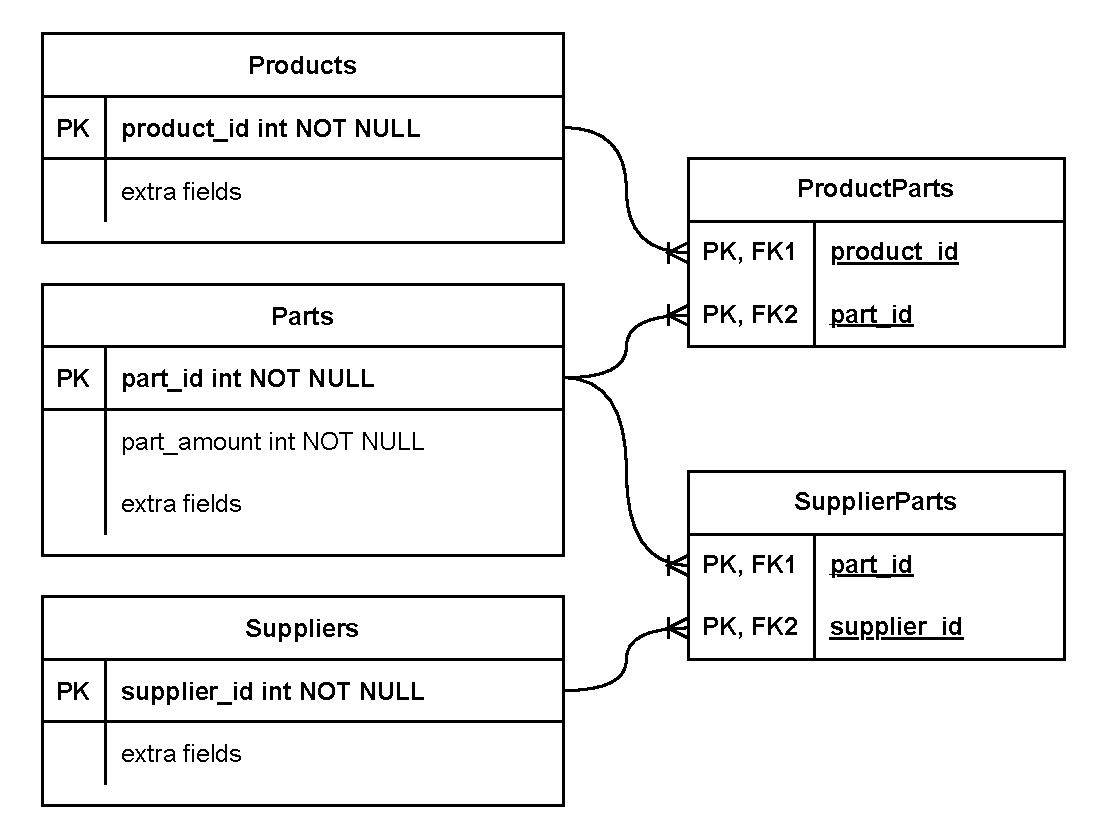
\includegraphics[width=1\linewidth]{figures/PPS ERD.pdf}
    \caption{Product-Parts-Supplier Entity Relationship Diagram.}
    \label{fig: pps-erd}
\end{figure}

The PPS workload has transactions with complex data dependencies that can lead to contention challenges when multiple transactions run concurrently. This complexity makes the workload suitable for evaluating how database systems handle the coordination and conflict resolution. The workload includes several types of transactions, namely:
\begin{itemize}
    \item \textit{OrderProduct}. Given a \texttt{product\_id}, this transaction will first collect the parts associated with the given product and then decrement the inventory amount for those parts. Importantly, this is a dependent transaction, since we do not know which parts will be updated in advance.
    \item \textit{GetPartsByProduct}. Given a \texttt{product\_id}, this transaction will retrieve the list of parts that are currently associated with the given product.
    \item \textit{UpdateProductPart}. Given \texttt{product\_id}, \texttt{part\_from}, and \texttt{part\_to}, this transaction will update a part associated with the given product by replacing the part identified with \texttt{part\_from} with the latter part \texttt{part\_to}.
    \item \textit{GetPart}. Given a \texttt{part\_id}, this transaction will retrieve the current inventory amount of the given part, along with any existing extra information.
    \item \textit{GetProduct}. Given a \texttt{product\_id}, this transaction will retrieve any extra information about the given product.
\end{itemize}

\section{Benchmark Implementation}
\label{sec: benchmark-implementation}
This section presents the implementation of our benchmarking framework, designed to evaluate the performance of geo-distributed transactional systems based on the PPS workloads. We discuss here key design choices, such as the integration of the benchmarking framework with the evaluated databases (Section~\ref{subsec: integration-with-different-databases}), the support for dependent transactions (Section~\ref{subsec: dependent-transactions}), the custom partitioning and home assignment schemes that offer precise control over transaction configurations (Section~\ref{subsec: partitioning-and-home-assignment-schemes}), and the transactional mix of the workload (Section~\ref{subsec: transactional-mix}).

\begin{figure}[ht]
    \centering
    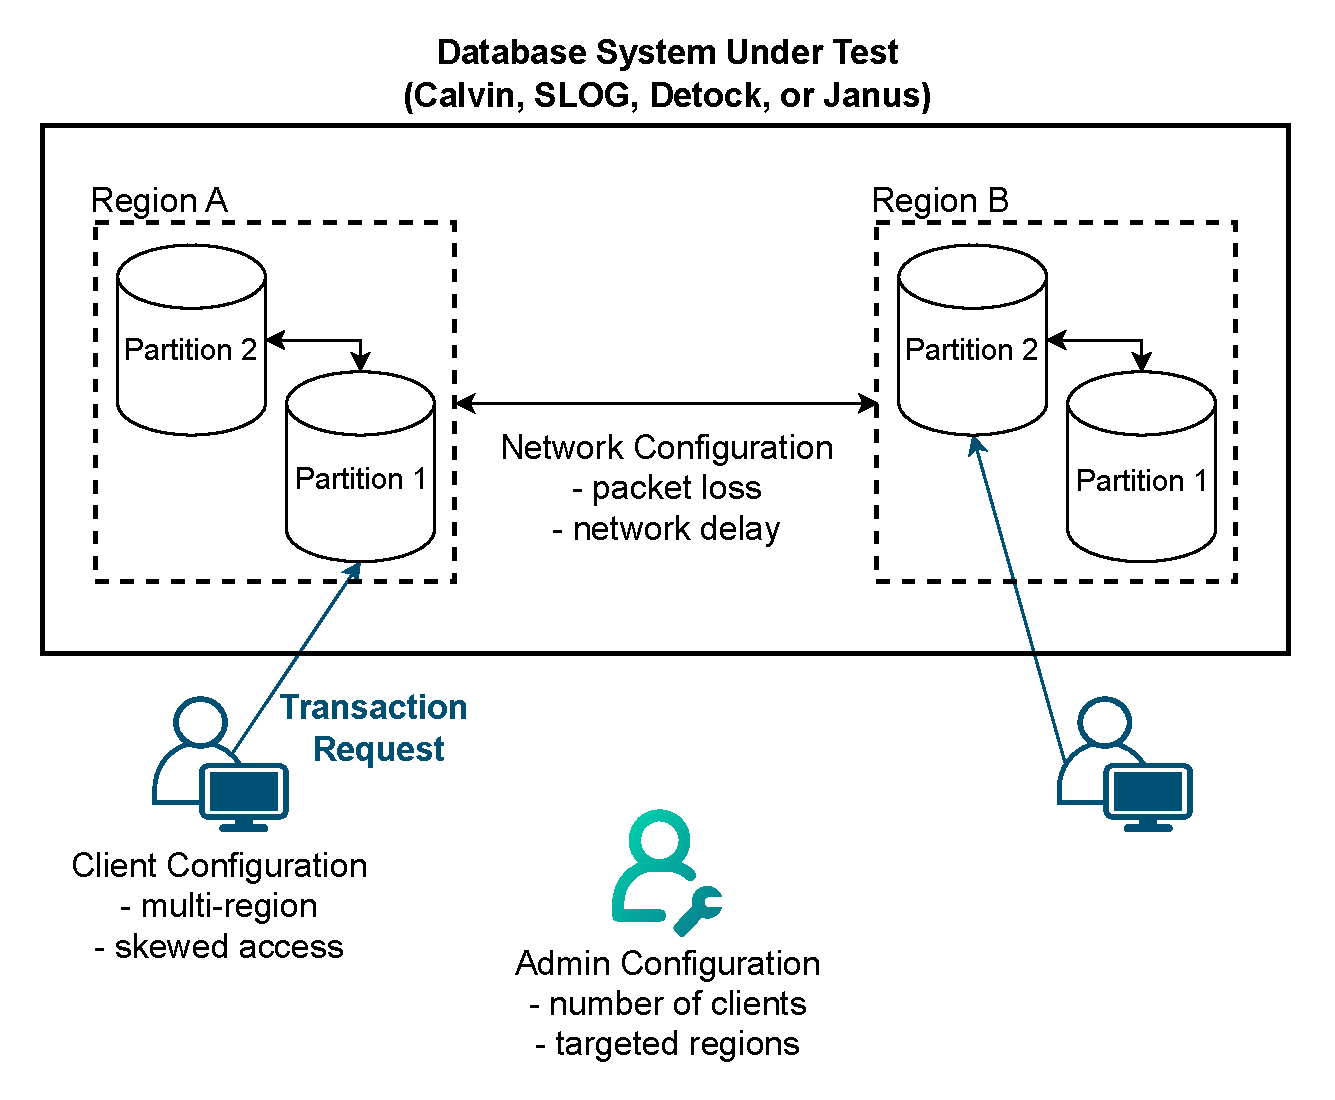
\includegraphics[width=1\linewidth]{figures/Overall Architecture.pdf}
    \caption{Architecture of the Benchmarking Framework, together with all the Tunable Parameters.}
    \label{fig: overall-architecture}
\end{figure}

\subsection{Integration with Different Databases}
\label{subsec: integration-with-different-databases}
The databases we evaluate follow a common setup, where data is partitioned across different servers, and each partition is replicated in different geographically distributed regions to ensure high availability and low latency by placing the data closer to the users. Our benchmark spawns client processes in different regions and can target specific partitions within any region. The architecture of our benchmarking framework and the way it interacts with the databases is shown in Figure~\ref{fig: overall-architecture}.

As stated in Section~\ref{subsec: evaluated-systems}, we implemented the benchmark within the Detock codebase to offer a unified testing environment for all the evaluated systems. This integration also allows us to define key components such as table schemas, table loaders, and stored procedures in a single place and use them consistently across all databases.

\subsection{Dependent Transactions}
\label{subsec: dependent-transactions}
As mentioned in Section~\ref{subsec: evaluated-systems}, all the evaluated databases need to know the complete set of accessed records for each transaction to either deterministically order them or construct the serialization graph. Among the transactions of the PPS workload, only \textit{OrderProduct} is a dependent transaction since it must first determine which parts are associated with the product before any updates can take place.

In its original design, Calvin was implemented to support dependent transactions by using a scheme called Optimistic Lock Location Prediction (OLLP) that makes use of a reconnaissance query to perform all the necessary reads to compute the complete read/write set before the actual execution begins. Unfortunately, this mechanism is not currently implemented in the Detock framework. As a solution, we will use a similar approach by splitting the \textit{OrderProduct} transaction into \textit{two client-side phases}. In the first phase, the client fetches the current list of parts associated with the given product. Then, in the second phase, the client issues the update request with the complete set of accessed records. It is important to note that when the second phase detects any changes in the reads done by the first phase, it will self-abort.

\subsection{Partitioning and Home Assignment Schemes.}
\label{subsec: partitioning-and-home-assignment-schemes}
Our benchmark supports custom partitioning schemes. In our setup, we partitioned the data across nodes in a round-robin fashion based on the record identifier (\texttt{product\_id}, \texttt{part\_id}, \texttt{supplier\_id}) for the core entities, and the \texttt{product\_id} for the two additional relationship tables. We say that a transaction is \textit{single-partition} if it accesses data from only one partition, and \textit{multi-partition} if it spans multiple partitions.

In addition to partitioning, SLOG and Detock use a couple of optimizations based on the concept of \textit{home regions}. In short, each record is assigned to exactly one geographical region, which is called the home region of this record and is responsible for coordinating the access to that record. Both systems assume that, theoretically, within each region, data is partitioned locally regardless of which region owns the data. This means that a single partition can hold records whose home regions are different. Similar to partitioning, we can classify the transactions into \textit{single-home} and \textit{multi-home}. Our implementation supports custom home assignment schemes. In our evaluation, we assign home regions in a round-robin fashion within each partition.

In our workload, only the second phase of the \textit{OrderProduct} transaction can be configured to be either single-partition or multi-partition, and independently, single-home or multi-home, depending on which parts are involved. The other transactions are simpler, since they either access only one record or all the accessed records fall within a single partition and home region, according to the chosen partitioning and home assignment scheme. The main challenge in configuring the second phase of the \textit{OrderProduct} transaction is that we do not know which parts will be accessed in advance. To overcome this, when creating the tables, we split the products into four groups based on the distribution of their parts:
\begin{itemize}
    \item \textit{Category I}. All parts are located in the same partition and have the same home region as the product itself.
    \item \textit{Category II}. All parts are located in the same partition as the product, but belong to different home regions.
    \item \textit{Category III}. All parts have the same home region as the product, but are located in different partitions.
    \item \textit{Category IV}. The parts are located in different partitions and also belong to different home regions.
\end{itemize}

By organizing the parts into these four categories, the benchmarking framework can dynamically generate \textit{OrderProduct} transactions with specific characteristics. For example, if we want to generate a single-home multi-partition transaction, we select a product from \textit{Category III}.

\subsection{Transactional Mix}
\label{subsec: transactional-mix}
Section~\ref{subsec: product-parts-supplier-workload} introduced the type of transactions that we consider in our benchmarking framework. While all these transactions reflect realistic business operations, such as updating a product or retrieving a part, not all of these types are well-suited for evaluating geo-distributed behavior. In particular, as stated in the previous subsection, only the \textit{OrderProduct} transaction has an access pattern that can span multiple partitions and regions, making it the only meaningful operation that can test the servers' coordination.

As a consequence, we used a transactional mix that favors the \textit{OrderProduct} type. In addition, we assigned greater weights to the \textit{UpdateProductPart} type, since it can interfere with two-phase dependent transactions, and to the \textit{GetPartsByProduct} type, since it accesses multiple records, making it more relevant for evaluating concurrency behavior. In contrast, the simple read-only transactions \textit{GetPart} and \textit{GetProduct} have lower priority. Table~\ref{tab: pps-transactional-mix} summarizes the mix.

\begin{table}[htbp]
  \centering
  \begin{tabular*}{\linewidth}{@{\extracolsep{\fill}} l r}
    \toprule
    \textbf{Transaction Type} & \textbf{Ratio} \\ \midrule
    \textit{OrderProduct} & 80\% \\
    \textit{GetPartsByProduct} & 8\% \\
    \textit{UpdateProductPart} & 8\%  \\
    \textit{GetPart} & 2\%  \\
    \textit{GetProduct} & 2\%  \\ \bottomrule
  \end{tabular*}
  \caption{PPS Transactional Mix used in our Experiments.}
  \label{tab: pps-transactional-mix}
\end{table}

% \section{Methodology, Background, Problem Description}
Choose one that fits your research best:
\subsection{Methodology and/or background}
Typically in general research articles, the second section contains a description of the research methodology, explaining what you, the researcher, is doing to answer the research question(s), and why you have chosen this method.
For purely analytical work this is a description of the data collection or experimental setup on how to test the hypothesis, with a motivation.

In any case this section includes references to necessary background information.
For a survey paper this includes the method of how you arrived at the set of papers included in the survey.

\subsection{Formal Problem Description}
For some types of work in computer science the methodology is standard: analyze the problem (e.g., make assumptions and derive properties), present a new algorithm and its theoretical background, proving its correctness, and evaluate unproven aspects in simulation.
Then an explanation of the methodology is often omitted, and the setup of the evaluation is part of a later section on the evaluation of the ideas.\footnote{This already shows that there is no single outline to be given for all papers.}
In this case, explain relevant (background) concepts, theory and models in this section (with references) and relate them to your research question.
Also this section then typically contains a more precise, formal description of the problem.

Do not forget to give this section another name, for example after the problem you are solving.


% \section{Your contribution (replace this section title by something more informative)}
In computer science typically the third section contains an exposition of the main ideas, for example the development of a theory, the analysis of the problem (some proofs), a new algorithm, and potentially some theoretical analysis of the properties of the algorithm.

Do not forget to give this section another name, for example after the method or idea you are presenting.

Some more detailed suggestions for typical types of contributions in computer science are described in the following subsections.


\subsection*{Experimental work}
In this case, this section will mostly contain a description of the methods/algorithms you will be comparing. Although not all methods need to be described in detail (providing appropriate references are available), make sure that you reveal sufficient details to a reader not familiar with these methods to: a) obtain a high-level understanding of the method and differences between them, and b) understand your explanation of the results/conclusions.

\subsection*{Improvement of an idea}
In this case, you would need to explain in detail how the improvement works. If it is based on some observation that can be proven, this is a good place to provide that proof (e.g., of the correctness of your approach). 

\subsection*{Literature survey}
If your contribution is a literature survey, then the organization of these ``middle'' sections very much depends on the way you want to present/organize the literature you are discussing.
First try to cluster papers that are similar in some aspect. Then think of how these clusters are related, from that you can think of a good order to discuss these clusters; this is sometimes called a bottom-up approach to writing a paper.

In addition, you may try to think about the organization of the literature from a top-down perspective: try to ``take a step back'' and think about the field and what important questions/variants are and build a hierarchical categorization of the field.

Make clear what your contribution is here: a new organization of the literature, identification of open problems/challenges, new parallels/generalizations, a table with pros/cons of different methods, etc.\ 



\begin{figure*}[t]
    \centering
    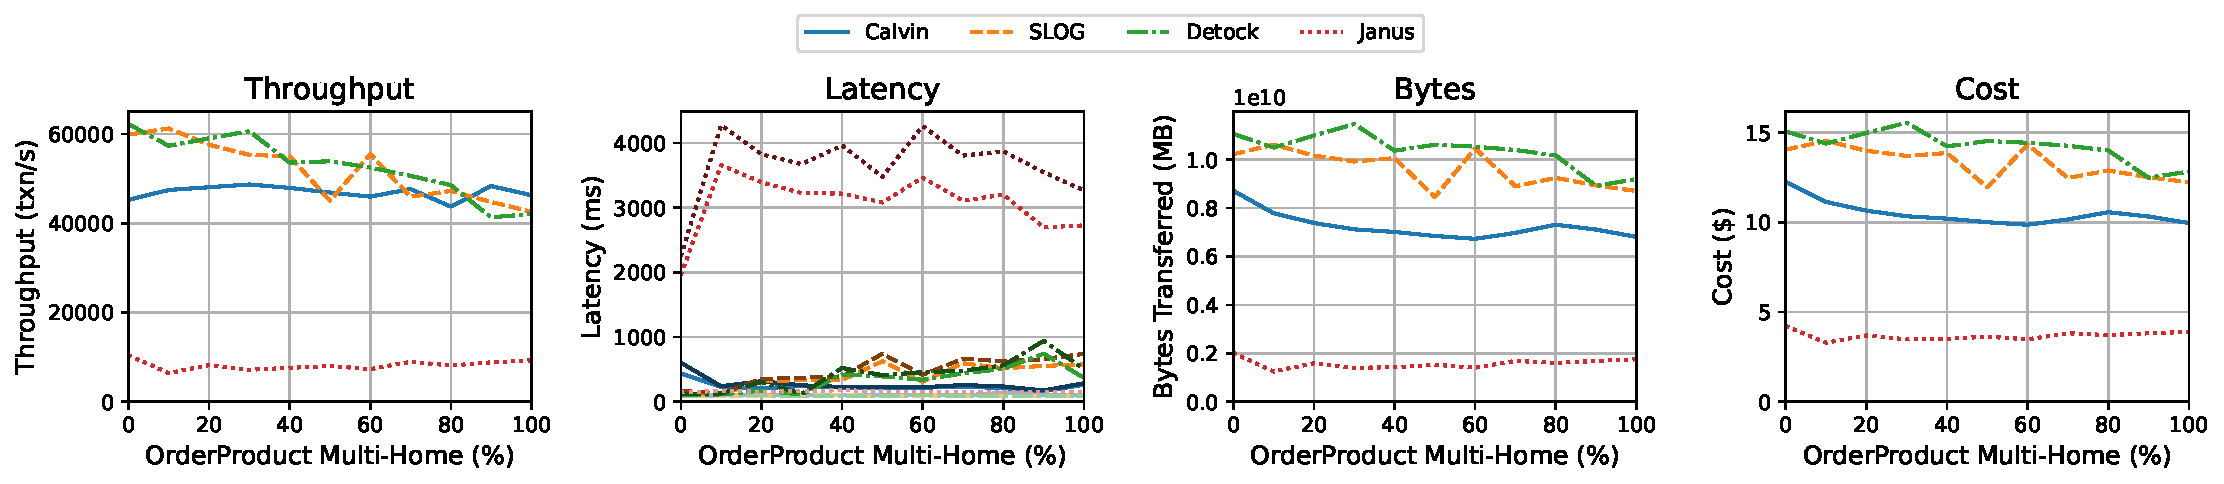
\includegraphics[width=1\textwidth]{figures/Baseline.pdf}
    \caption{Results of the Baseline Scenario.}
    \label{fig: baseline-scenario}
\end{figure*}

\begin{figure*}[t]
    \centering
    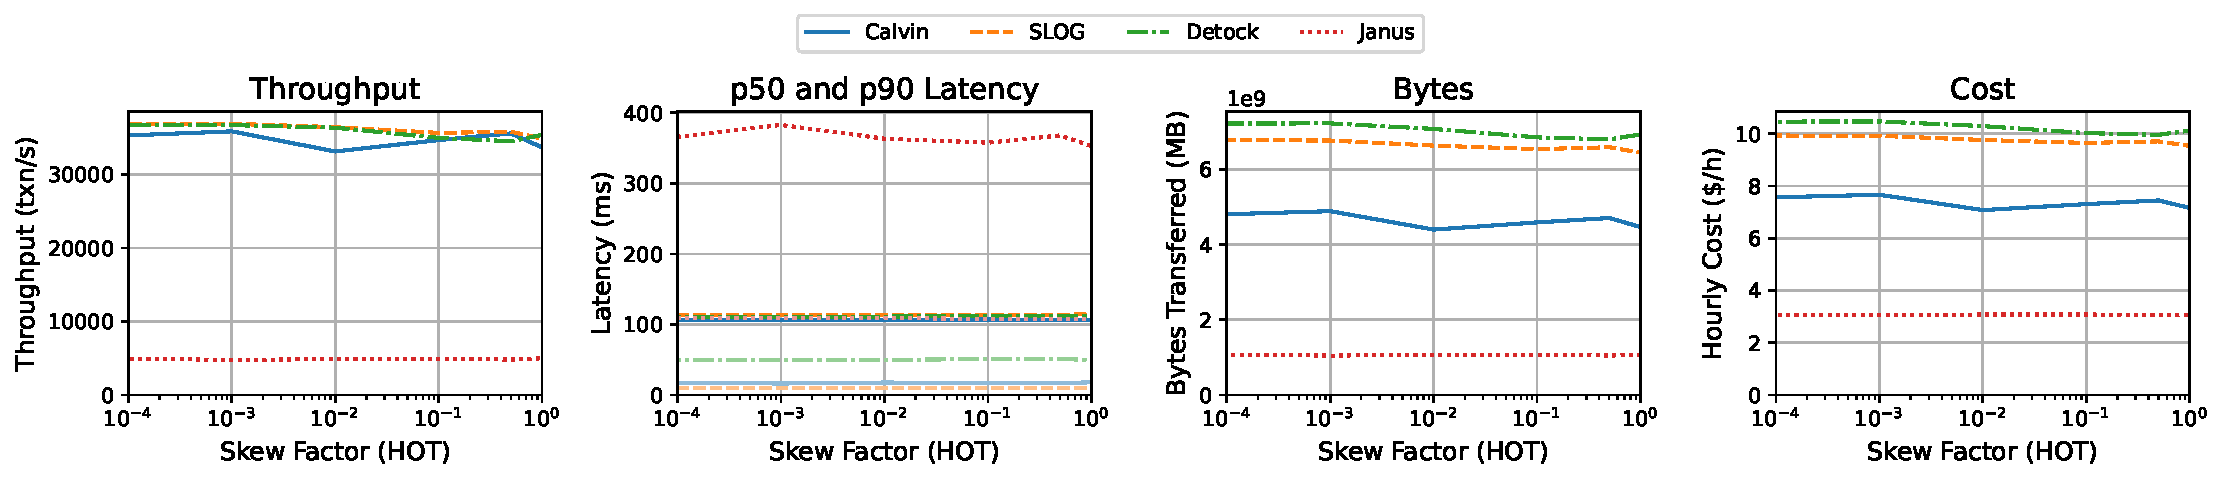
\includegraphics[width=1\textwidth]{figures/Skew.pdf}
    \caption{Results of the Skew Access Scenario.}
    \label{fig: skew-access-scenario}
\end{figure*}

\section{Experimental Setup and Results}
\label{sec: experimental-setup-and-results}
This section outlines our experimental methodology and key findings. Section~\ref{subsec: deployment-and-metrics-collection} describes our deployment setup and the methodology used for performance measurement, and Section~\ref{subsec: evaluation-scenarios-and-results} presents the results obtained under a range of different experimental scenarios.

\subsection{Deployment and Metrics Collection}
\label{subsec: deployment-and-metrics-collection}
We conducted all experiments on a dedicated 4-node high-performance cluster located in our university. Each node is equipped with dual AMD EPYC 7H12 processors, 256 hardware threads, and 503 GiB of RAM. The nodes are interconnected via 10 Gigabit Ethernet.

In our experiments, we simulated a two-region deployment by using all four physical nodes and injecting artificial network delay between them. Both clients and servers are deployed as Docker containers to ensure a clean and reproducible environment. Figure~\ref{fig: overall-architecture} illustrates the setup. The data is divided into two partitions, and each logical region consists of two server containers that hold a complete copy of both partitions. The cluster delivers a natural intra-region round-trip time (RTT) of roughly 0.15 ms, and we set the inter-region RTT to 100 ms (Table~\ref{tab: rtt-machines}).

\begin{table}[htbp]
  \centering
  \begin{tabular*}{\linewidth}{@{\extracolsep{\fill}} l r r r r}
    \toprule
               & \textbf{A-P1} & \textbf{A-P2} & \textbf{B-P1} & \textbf{B-P2} \\ \midrule
    \textbf{A-P1} & —      & 0.15 ms & 100 ms & 100 ms \\
    \textbf{A-P2} & —      & —      & 100 ms & 100 ms \\
    \textbf{B-P1} & —      & —      & —      & 0.15 ms \\
    \textbf{B-P2} & —      & —      & —      & —      \\ 
    \bottomrule
  \end{tabular*}
  \caption{Round-trip times between all unordered pairs of machines. We uniquely identify the machines with the label \textit{Region-Partition} (e.g., \textit{A-P1} is the partition 1 within the region A).}
  \label{tab: rtt-machines}
\end{table}

Unless stated otherwise, the clients are uniformly distributed across the two regions. To avoid overwhelming or underdriving the systems, we first explore the effects of the number of clients using the scalability test from Section~\ref{subsubsec: scalability-scenario}. We identify for each system the point where additional clients would no longer increase the throughput, and use that client count in all remaining scenarios.

For performance evaluation, each client container collects local metrics during execution, which are then aggregated by a centralized admin. The metrics we focus on are throughput, latency, abort rates, and bytes transferred, and we also estimate the operational cost. Throughput, latency, and abort rates are measured directly by the application logic, while the number of transferred bytes is collected using system-level network monitoring tools. Additionally, we provide a simplistic estimation of the operational cost by monitoring the resource utilization within the server containers and tracking the overall network usage. The formula we use for the hourly cost is $C = N_{\text{machine}} * P_{\text{machine}} + V_{\text{traffic}} * P_{\text{traffic}}$, where $N_{\text{machine}}$ is the number of server containers, $P_{\text{machine}}$ is the on-demand hourly price for the each used machine, $V_{\text{traffic}}$ is the cross-region traffic volume, and $P_{\text{traffic}}$ is the data transfer price.

\subsection{Evaluation Scenarios and Results}
\label{subsec: evaluation-scenarios-and-results}
We now describe the experimental scenarios used in our evaluation. We designed these scenarios to systematically observe the impact of different system configurations on the transactional performance of the database systems. Each scenario is strongly connected with the tunable parameters shown in Figure~\ref{fig: overall-architecture}, which control the network conditions, the clients' placement, and the transactional load.

\subsubsection{Baseline Scenario}
\label{subsubsec: baseline-scenario}
In the baseline scenario, we aim to understand how each concurrency control protocol performs under standard conditions in the two-region deployment with no artificial skew, packet loss, or extra delay besides the default link latencies shown in Table~\ref{tab: rtt-machines}. Specifically, we vary only the fraction of \textit{multi-home transactions} among the \textit{OrderProduct} type while keeping the proportion of multi-partition transactions constant at 50\%. This scenario allows us to isolate the cost of coordination across different geographical regions. Figure~\ref{fig: baseline-scenario} shows the metrics collected for each protocol: the throughput, the median latency ($p50$), along with the $90^{th}$-percentile latency ($p90$), the bytes transferred, and the hourly operational cost.

Among all systems, Janus has the lowest throughput and the highest latencies. This is primarily because Janus does not have the notion of multi-home transactions, and routes every commit through its integrated consensus path, which requires cross-region coordination even for transactions that could be executed locally. As a consequence, the throughput stays constant, and even the single-region transactions need at least one WAN round-trip, which is visible in the plot as the $p50$ latency sits near the inter-region RTT ($\approx$100 ms). In case of conflicts, Janus needs an additional wide-area round-trip, so $p90$ latency exceeds 200 ms, and even slightly increases with larger MH fractions, since this inherently increases the contention, as the regions will contend for the same products.

Calvin also does not have the notion of multi-home transactions, and thus, the throughput stays almost constant. It performs worse than SLOG and Detock when the proportion of multi-home transactions is low, but it overtakes them as the proportion exceeds roughly $60\%$. This is because Calvin relies on a deterministic global sequencer that orders all transactions. When most transactions are local, Calvin's overhead for global ordering becomes unnecessary and costly, but as the proportion of multi-home transactions increases, Calvin's global sequencer can coordinate them efficiently and get a better performance than SLOG and Detock, which incur a significant cost of handling multi-home transactions.

\subsubsection{Skewed Access Scenario}
\label{subsubsec: skew-access-scenario}
In the skewed access scenario, we study how each protocol handles the contention caused by an uneven access pattern. We fix the workload composition so that half of the \textit{OrderProduct} transactions are multi-home, and similarly, half of them are multi-partition. To introduce skew, we use the NURand distribution to define so-called \textit{hot records} that will be accessed more often depending on the \textit{skew factor} \cite{council2010tpc}.

As shown in Figure~\ref{fig: skew-access-scenario}, the curves remain nearly flat for all four systems across the entire range of skew factors. For the deterministic designs (Calvin, SLOG, Detock), this is expected since each replica already knows the global order before the execution begins, so a hot key cannot block related transactions. The skew also has little effect on Janus, showing that the system's bottleneck is given by the WAN round-trip.

\begin{figure*}[ht]
    \centering
    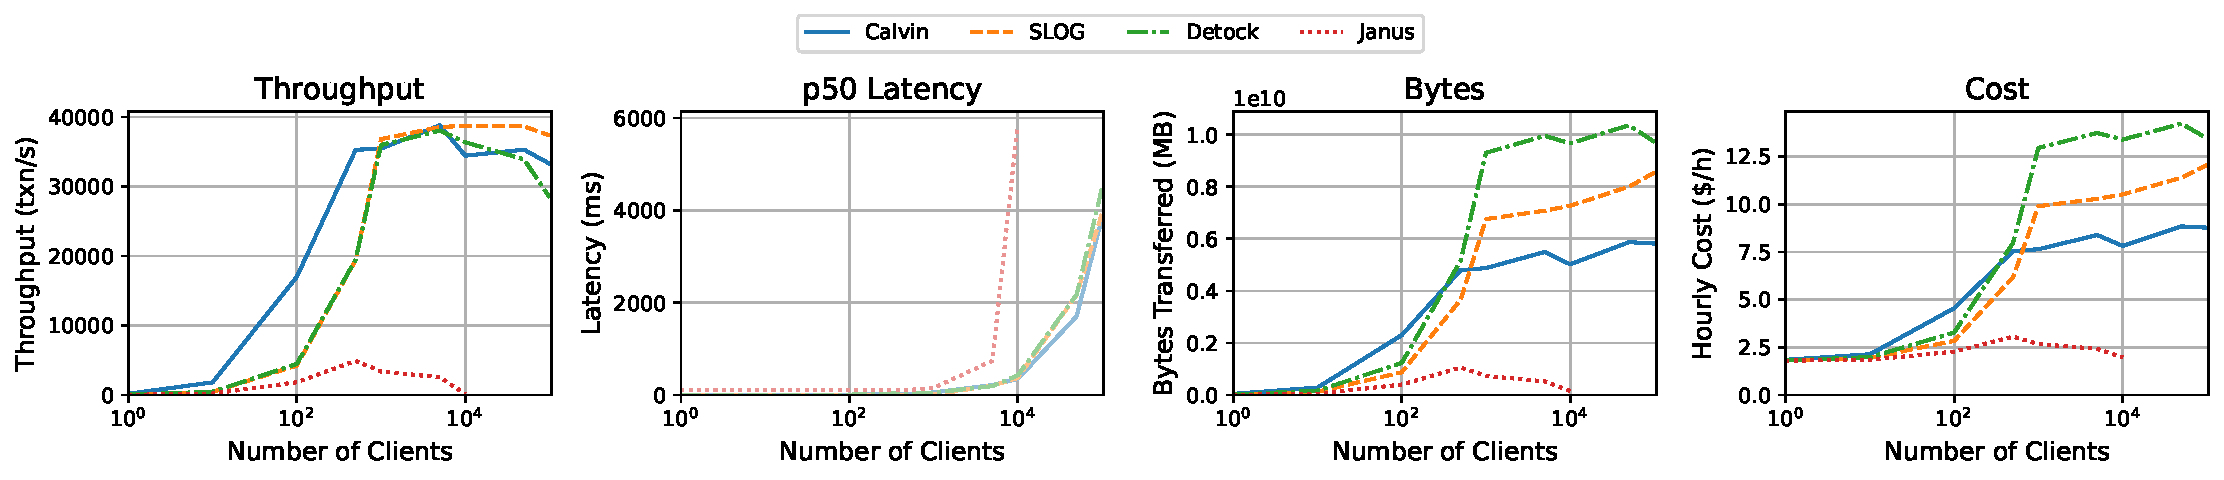
\includegraphics[width=1\textwidth]{figures/Scalability.pdf}
    \caption{Results of the Scalability Scenario.}
    \label{fig: scalability-access-scenario}
\end{figure*}

Figure~\ref{fig: abort-rates} reveals the hidden cost of the skew. The protocols themselves don't abort transactions, since Calvin, SLOG, and Detock commit every transaction in the predetermined order, and Janus commits according to the serialization graph. Therefore, all aborts we observe come from the way we execute the dependent transaction \textit{OrderProduct}. We split it into a read-only phase that retrieves the parts currently associated with the given product, and a write phase that performs the updates. If any of those parts change between those two phases, the server aborts the second phase and signals the client to retry the whole transaction starting from the first phase. The presence of hot records raises the chance that the second phase's validation fails, which explains why abort rates increase with the skew for all systems. However, the increase is small, peaking at only $2.5\%$ among all systems, and leaving throughput and latency practically unchanged.

\begin{figure}[ht]
  \centering
  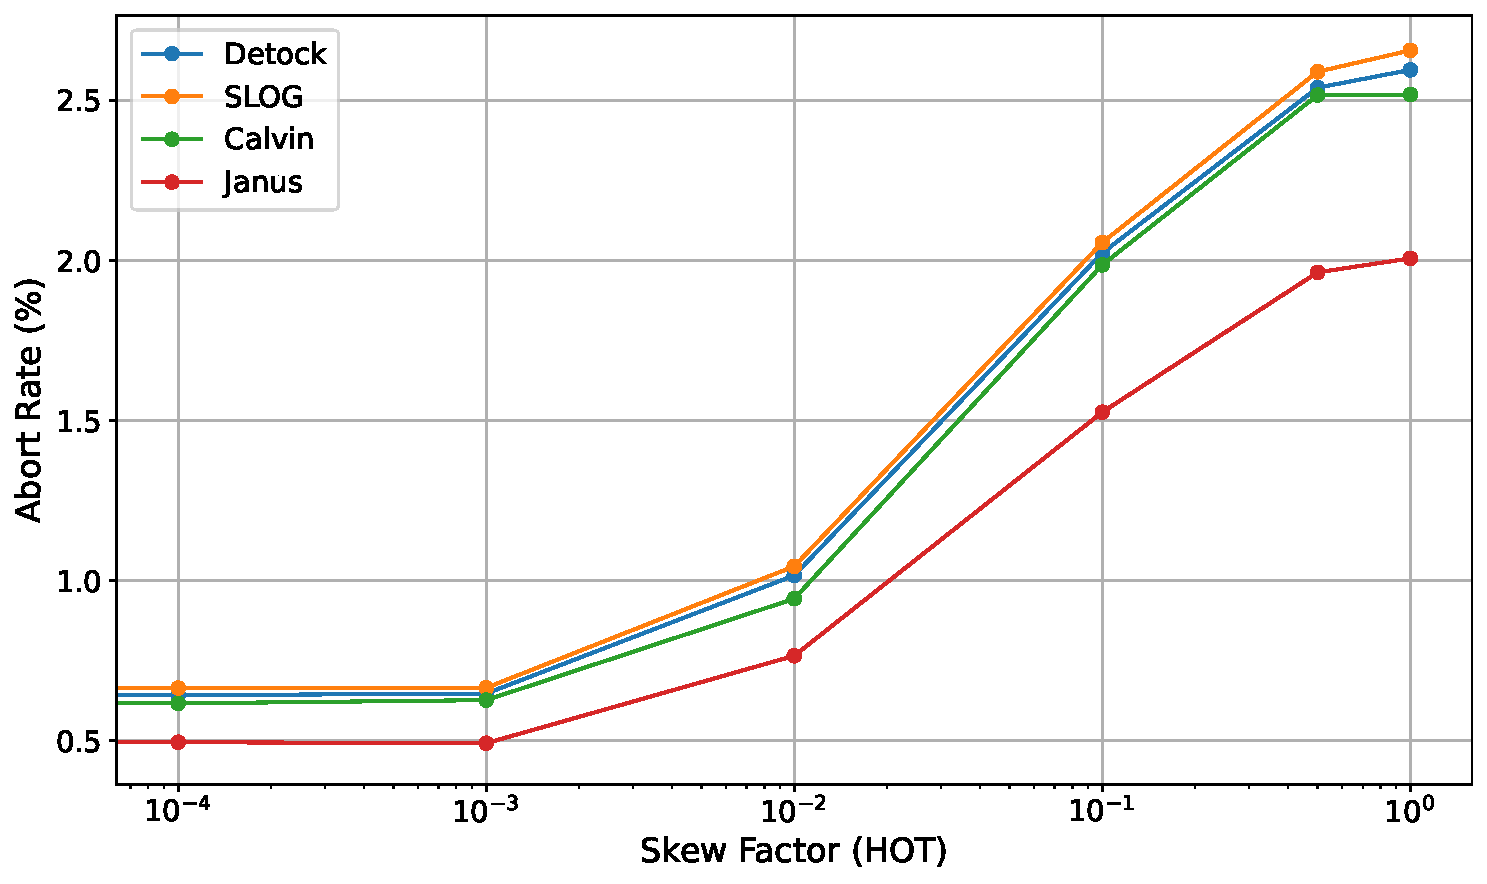
\includegraphics[width=\columnwidth]{figures/Abort Rates.pdf}
  \caption{Abort Rates in the Skew Access Scenario.}
  \label{fig: abort-rates}
\end{figure}

\subsubsection{Sunflower Topology Scenario}
\label{subsubsec: sunflower-topology-scenario}
The sunflower experiment analyzes how the protocols react when one region turns into a central hub. This is a common occurrence in the real world, where deployments rarely receive perfectly balanced traffic. A viral event, a seasonal sale, or an outage in a neighboring zone can redirect requests into one data centre while the others stay idle. To reproduce this, we perform a 100-second run, where we start with balanced traffic, and then linearly increase the share of transactions whose home region is \textit{Region A} (or, for multi-home transactions, include \textit{Region A} in the home set) with 10\% every 10 seconds, until it receives the entire load. Throughout the experiment, we keep the workload mix fixed at $50\%$ multi-partition and $50\%$ multi-home transactions, and leave the default RTTs unchanged, so any throughput change reflects only the growing regional imbalance.

Figure~\ref{fig: sunflower-throughput} plots the resulting throughput. At the start, when traffic is evenly split, all systems have their baseline throughput. As the bias grows, SLOG and Detock are the only ones that experience a decrease in throughput. Once more requests land in the same region, the single-home fast path overwhelms the replica while its counterpart in \textit{Region B} sits mostly idle, so the aggregate throughput drops.

In contrast, Calvin's throughput stays approximately the same. In the Detock codebase, Calvin's global sequencer uses a replication based on a primary replica by asynchronously sending every transactional input (both the single-home and multi-home transactions) to a dedicated region that broadcasts the batches in order. Since the primary replica already acts as a central point, increasing the bias doesn't have an effect on the overall throughput. Similar to the skew access scenario (\ref{subsubsec: skew-access-scenario}), Janus once again shows the lowest absolute throughput, but it is practically insensitive to the bias. Every commit must gather a WAN approval, so moving clients from \textit{Region A} to \textit{Region B} doesn't affect the throughput.

\begin{figure}[ht]
  \centering
  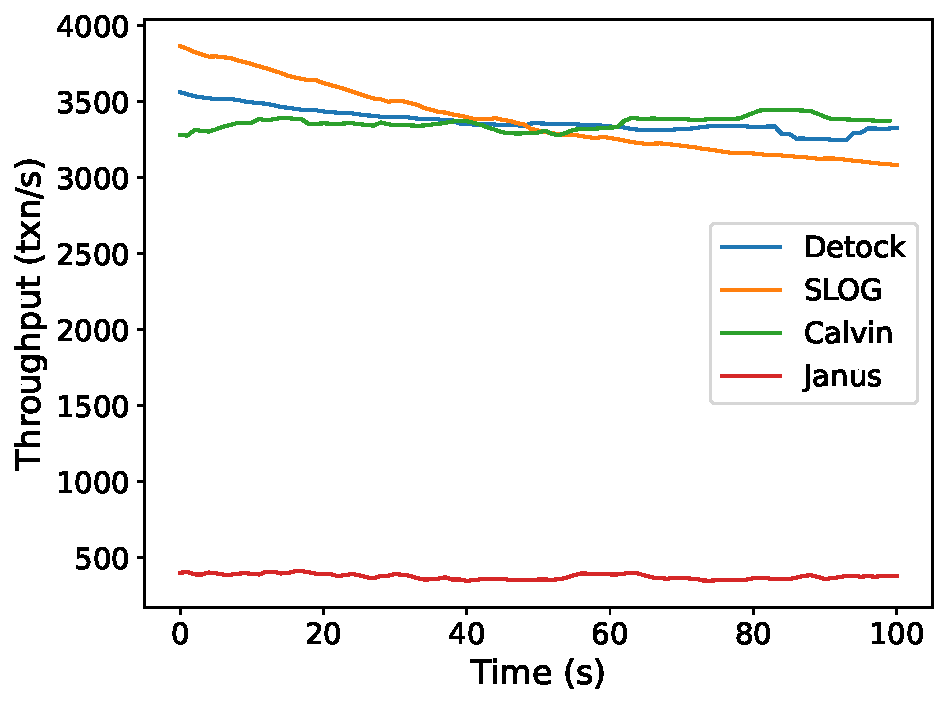
\includegraphics[width=\columnwidth]{figures/Sunflower Throughput.pdf}
  \caption{Throughput in the Sunflower Topology Scenario.}
  \label{fig: sunflower-throughput}
\end{figure}

\begin{figure*}[ht]
    \centering
    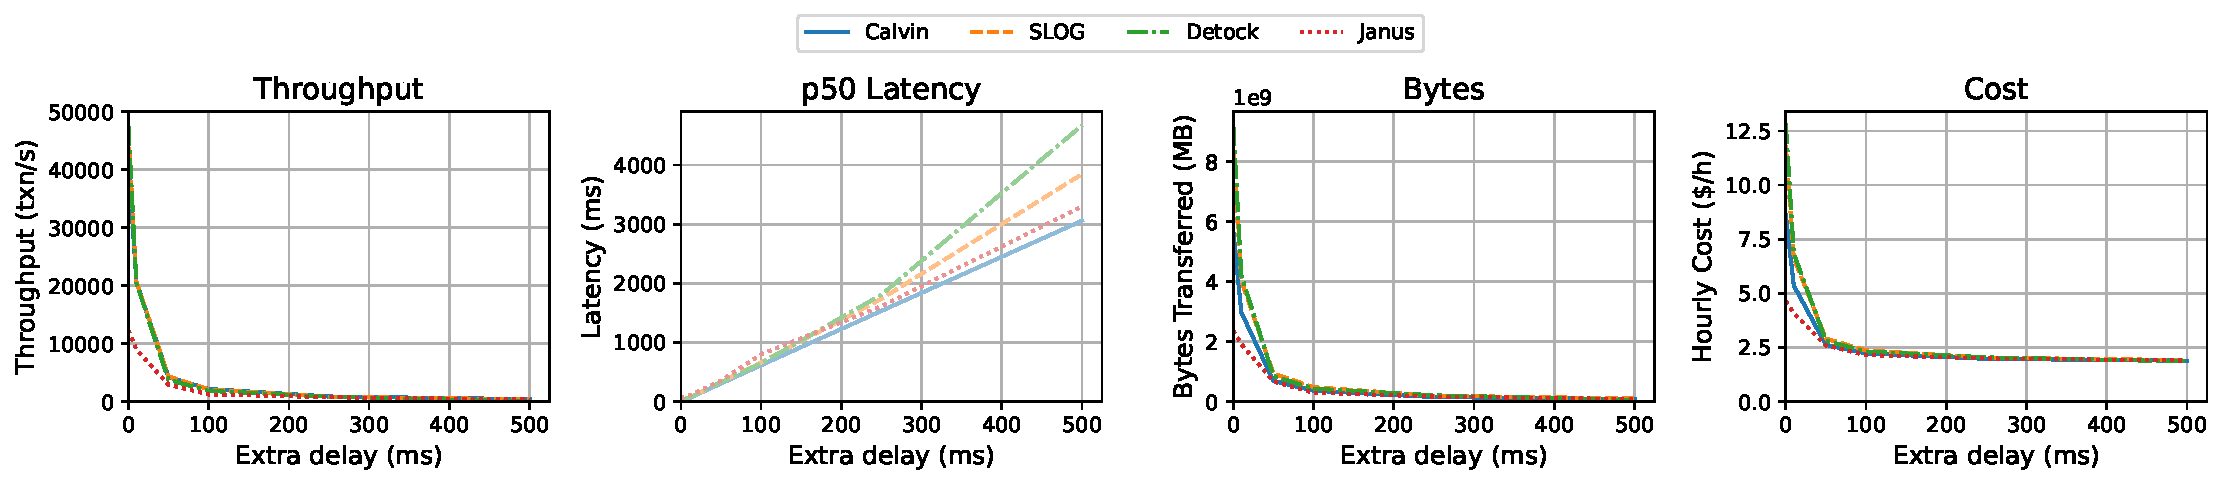
\includegraphics[width=1\textwidth]{figures/Network.pdf}
    \caption{Results of the Network Delays Scenario.}
    \label{fig: network-delays-scenario}
\end{figure*}

\begin{figure*}[ht]
    \centering
    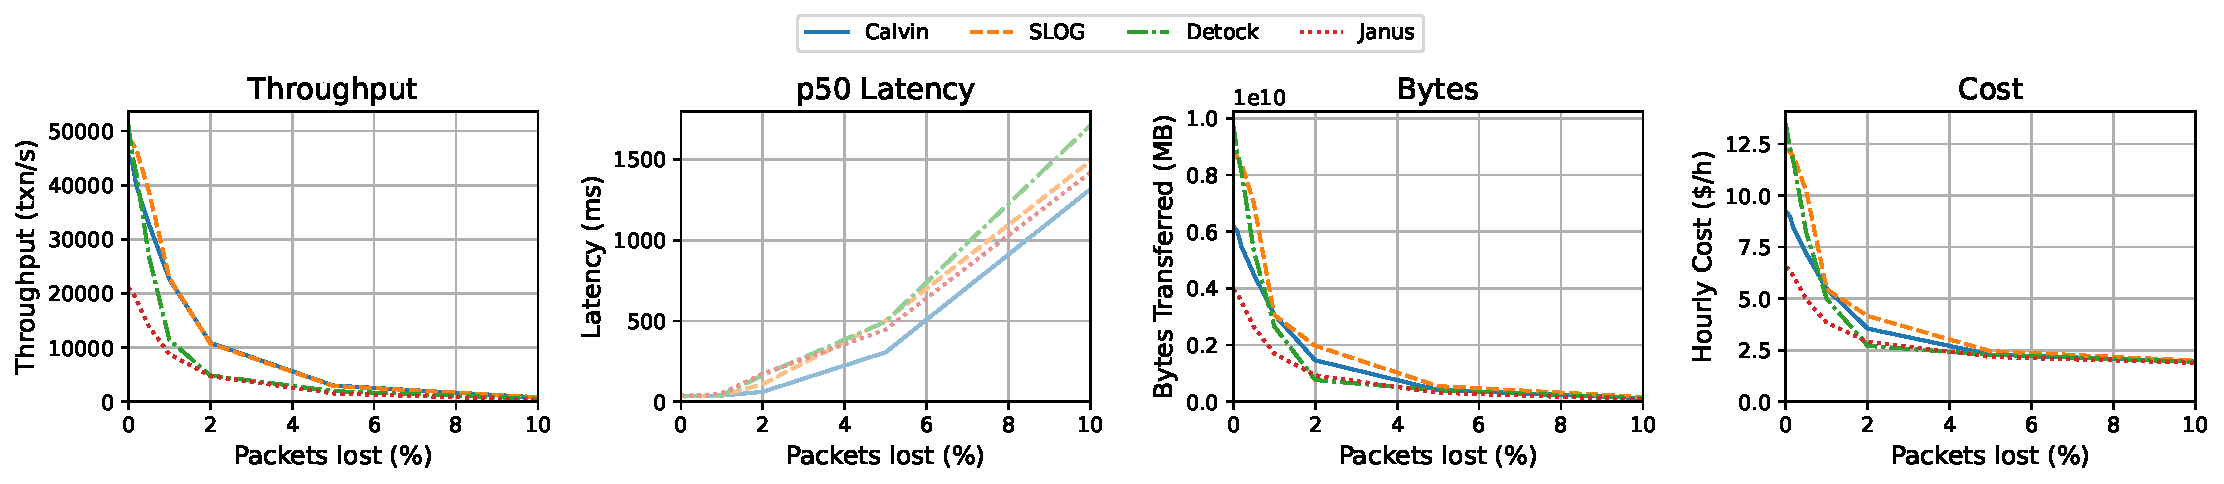
\includegraphics[width=1\textwidth]{figures/Packet Loss.pdf}
    \caption{Results of the Packet Loss Scenario.}
    \label{fig: packet-loss-scenario}
\end{figure*}

\subsubsection{Scalability Scenario}
\label{subsubsec: scalability-scenario}
The scalability scenario focuses on evaluating how each protocol performs as we increase the number of clients, while keeping the workload composition fixed at its standard configuration with $50\%$ multi-home transactions, $50\%$ multi-partition transactions, and no added skew. Figure~\ref{fig: scalability-access-scenario} shows how SLOG, Detock, and Calvin all have similar improvements in throughput as the load increases, which demonstrates that these systems have good scalability given a balanced transactional workload. Janus, on the other hand, scales to roughly 1000 clients, then its throughput collapses to 0. The likely reason is that Janus's unified consensus and replication layer has to handle more and more dependency checks in the serialization graph, which overwhelms its CPUs and network links until it can no longer make progress.

\subsubsection{Network Delays Scenario}
\label{subsubsec: network-delays-scenario}
This scenario explores how extra latency affects each system. We inject an additional delay on every cross-region link while keeping the packet loss at $0\%$ and using the standard workload mix from Section~\ref{subsubsec: scalability-scenario}. Figure~\ref{fig: network-delays-scenario} plots the results. The throughput decreases exponentially for all systems as the round-trip time grows. We note that the median latencies increase linearly with the injected delay, and Calvin's latency curve remains the lowest. This indicates that Calvin uses the smallest number of messages per transaction. Indeed, the coordinator only forwards the transactional input to the primary replica, which then broadcasts the messages in order. 

\subsubsection{Packet Loss Scenario}
\label{subsubsec: packet-loss-scenario}
In this experiment, we inject random packet loss on the WAN links, ranging from $0\%$ to $10\%$, while leaving the RTTs at their default values and the workload mix at its standard from Section~\ref{subsubsec: scalability-scenario}. Once again, the throughput falls exponentially for all systems, and Calvin proves itself the most resilient in terms of latency. This again proves Calvin's lightweight communication, which minimizes the number and size of WAN messages that can be delayed or lost.

\section{Responsible Research}
\label{sec: responsible-research}
This work does not involve personal data or any ethically sensitive information. We conducted all the experiments using synthetic data, which does not come from real users or real-world systems. Because of this, there are no ethical concerns related to privacy or security in our research.

We made efforts to ensure the reproducibility of our results. Section~\ref{subsec: deployment-and-metrics-collection} describes the environment used for the experiments, along with the way we measured the performance and collected the metrics. The deployment is fully automated using Docker containers. The source code for the server, client, and experimental scripts will be available in a public repository\footnote{\url{https://github.com/delftdata/Detock}}, along with step-by-step instructions for setting up the benchmarking framework, running the experiments, and collecting the results. We understand that others who repeat our experiments may get slightly different results. This is expected in distributed systems research due to several factors, including the noise from background processes or the unpredictability of network communication. To reduce this variability, we ran the experiments several times and reported the average result. This helps in making our comparisons more reliable. In addition, we used fixed random seeds in our transaction generator, so that experiments with identical parameters follow the same behavior across different runs.

\section{Discussion}
\label{sec: discussion}
Our experiments show that the PPS workload complements the commonly used workloads TPC-C and YCSB+T by covering several gaps they leave open, but it doesn't address every evaluation need. In this section, we outline the main advantages of using the PPS workload (Section~\ref{subsec: advantages-of-the-pps-workload}) and also acknowledge its limitations (Section~\ref{subsec: limitations-of-the-pps-workload}).

\subsection{Advantages of the PPS Workload}
\label{subsec: advantages-of-the-pps-workload}
\paragraph{Dependent Transactions.}
PPS models many-to-many relationships between products, parts, and suppliers. Thus, transactions need to work with \textit{foreign key dependencies} when joining different tables, which is not the case in the single-table YCSB+T workload and the TPC-C warehouse hierarchy. In particular, the \textit{OrderProduct} type needs to perform a read phase to discover all the relevant parts before being able to perform the actual updates. If another client changes the retrieved list of parts in between, then the transaction aborts and retries. Neither TPC-C nor YCSB+T ever forces the systems to abort, so PPS is the only one of these three workloads that stresses this case. We captured how increasing the skew factor impacts the resulting abort rates in Section~\ref{subsubsec: skew-access-scenario}.

\paragraph{Longer Transaction Footprint.}
PPS allows us to choose the number of parts per product, and thus control the size of the \textit{read/write sets} of both \textit{GetPartsByProduct} and \textit{OrderProduct} transactions. In our experiments, we set this parameter to 10. The larger access sets in PPS particularly penalize the protocols whose cross-region coordination grows in complexity as the number of keys increases. Janus is an example of such a design, where a larger access set would lead to bigger messages and more potential conflicts, which pushes the transaction on the slow path that needs a second WAN round-trip. As a consequence, Janus's throughput relative to the other systems in our PPS baseline (Section~\ref{subsubsec: baseline-scenario}) is far lower than in Nguyen et al.'s study \cite{nguyen2023detock}, which used YCSB+T.

\paragraph{Fine-grained Home Region Control.}
Besides the ability to dynamically generate multi-home or single-home transactions, which is a feature already available in the Detock performance evaluation \cite{nguyen2023detock}, our PPS-based benchmarking framework allows us to redirect a configurable fraction of transactions to a particular region. For a single-home transaction, we can select the exact region that will coordinate it, and for a multi-home transaction, we can pick a specific region to appear in the home set. This flexibility was essential for the sunflower experiment (Section~\ref{subsubsec: sunflower-topology-scenario}), where we gradually shifted the traffic to a region to create a realistic \textit{hotspot}.

\subsection{Limitations of the PPS Workload}
\label{subsec: limitations-of-the-pps-workload}
\paragraph{Limited Updates.}
Unfortunately, only two transactions in the PPS workload mix perform writes, namely \textit{OrderProduct} and \textit{UpdateProductPart}. Each of them modifies records from a \textit{single table}. On the other hand, TPC-C offers a broader spectrum of write patterns, which can lead to more interesting contention challenges that PPS cannot reproduce.

\paragraph{Multi-home and Multi-partition Limitations.}
Because only the \textit{OrderProduct} transaction can be configured to be multi-home or multi-partition, the workload mix must be adjusted to consider this. Even though we can choose the percentages of \textit{OrderProduct} transactions in the mix, it is still a dependent transaction whose read-only first phase is always single-home and single-partition, and thus we cannot achieve an \textit{overall combination} where $100\%$ of the generated transactions are multi-home and multi-partition. On the other hand, even though YCSB+T is simpler, it allows arbitrary key distributions, so it can be used to reach any desired proportion of multi-home and multi-partition transactions.

\section{Conclusions and Future Work}
\label{sec: conclusion-and-future-work}

This work introduced a configurable benchmarking framework based on the PPS workload and demonstrated how it can be used to augment the standard workloads TPC-C and YCSB+T. Our benchmark adds dependent transactions, larger read/write sets, and fine-grained control over single-home and multi-home access patterns, which are key aspects when evaluating any geo-distributed database system. 

Using this benchmark, we compared four such systems, Calvin, SLOG, Detock, and Janus, across six different scenarios. The results show clear tradeoffs. Calvin's global sequencer pays off once there's a majority of transactions that access multiple regions, whereas SLOG and Detock excel when most transactions can be executed locally. Janus's bottleneck is the required WAN round-trip approval, and the larger PPS access set can potentially lead to another WAN round-trip to solve the conflicts, which generally proved to have low performance in our two-region deployment. The skew experiment showed the hidden cost of having dependent transactions through increasing abort rates, while the sunflower experiment exposed how systems that are optimized based on locality can overload one replica.

Ultimately, the purpose of this paper is to raise awareness of the need for benchmarks suited for geo-distributed databases. Although PPS fills some gaps, it has its limitations. Future extensions could introduce additional transactions that are write-heavy or have the potential to span multiple regions. Moreover, it might be worth exploring how the results would be affected by having server-side reconnaissance (OLLP) for dependent transactions.

%DIF <  \appendix
\section{Further guidelines}

\subsection{Reference use, Tables, and Figures}
\begin{itemize}
    \item IEEE citation style [1].
    \item All tables and figures must be numbered and captioned.
    \item Introduce figures and tables in the body of text before actually using them.
    \item Tables and figures must be understandable and stand alone.
    \item Tables start and end with double horizontal lines.
    \item Tables have minimal column and row line separators.
    \item Table labels and titles are placed before the table.
    \item Figure labels and titles are placed after the figure.
\end{itemize}

\subsection{Writing Style and Language}
\begin{itemize}
    \item Paragraphs only treat a single idea and are clear and concise.
    \item Writing style is formal.
    \item Active voice is preferred; passive voice should be used sparingly.
    \item Colloquial speech, slang, and contractions shall not be used.
    \item The past tense is used for methods/results (already completed).
    \item The present tense is used for general facts and statements.
    \item Define acronyms at first use.
\end{itemize}
\DIFdelbegin %DIFDELCMD < 

%DIFDELCMD < %%%
\DIFdelend \bibliographystyle{IEEEtran}
\bibliography{references}
\DIFaddbegin 

\clearpage
\appendix
\section{\DIFadd{Use of Large Language Models}}
\DIFadd{In compliance with the }\textit{\DIFadd{Course Policy on the Use of Large Language Models (LLMs)}}\DIFadd{, LLMs were used exclusively for correcting the grammatical errors and improving the stylistic clarity, and not for generating ideas or drafting new text passages. The used prompts had the pattern: "Please provide feedback on the readability of the following paragraph: ..." and "Please fix the grammar in the following paragraph: ...".
}\DIFaddend 

\end{document}